\documentclass{article}
\usepackage[english, spanish]{babel}
\usepackage{float}
\usepackage[letterpaper, portrait, margin=2.54cm]{geometry} % Combinada y actualizada
\usepackage{graphicx}
\usepackage{lipsum}
\usepackage{amsmath,amssymb,amsthm}
\usepackage[utf8]{inputenc}
\usepackage{multirow}
\usepackage{csquotes}
\usepackage{apacite}
\usepackage{multicol}
\usepackage{parskip}
\usepackage{setspace}
\usepackage{empheq}
\usepackage{mdframed}
\usepackage{booktabs}
% \usepackage{lipsum} % Eliminado, ya cargado
% \usepackage{graphicx} % Eliminado, ya cargado
\usepackage{color}
\usepackage{psfrag}
\usepackage{pgfplots}
\usepackage{bm}
\usepackage{tocloft}
\usepackage{lscape}
\usepackage{adjustbox}
\setlength{\tabcolsep}{1.505625pt}
\renewcommand{\arraystretch}{1.2}
%%%%%%%%%%%%%%%%%%%%%%%%%%%%%%%%%%%%%%%%%%%%%%%%%%%%%%%%%%%%%%%%%%%%%%%%%%%%%%%
\definecolor{ocre}{RGB}{243,102,25}
\definecolor{mygray}{RGB}{243,243,244}
\definecolor{deepGreen}{RGB}{26,111,0}
\definecolor{shallowGreen}{RGB}{235,255,255}
\definecolor{deepBlue}{RGB}{61,124,222}
\definecolor{shallowBlue}{RGB}{235,249,255}
%%%%%%%%%%%%%%%%%%%%%%%%%%%%%%%%%%%%%%%%%%%%%%%%%%%%%%%%%%%%%%%%%%%%%%%%%%%%%%%

%%%%%%%%%%%%%%%%%%%%%%%%%% Define an orangebox command %%%%%%%%%%%%%%%%%%%%%%%%
\newcommand\orangebox[1]{\fcolorbox{ocre}{mygray}{\hspace{1em}#1\hspace{1em}}}
%%%%%%%%%%%%%%%%%%%%%%%%%%%%%%%%%%%%%%%%%%%%%%%%%%%%%%%%%%%%%%%%%%%%%%%%%%%%%%%

%%%%%%%%%%%%%%%%%%%%%%%%%%%% English Environments %%%%%%%%%%%%%%%%%%%%%%%%%%%%%
\newtheoremstyle{mytheoremstyle}{3pt}{3pt}{\normalfont}{0cm}{\rmfamily\bfseries}{}{1em}{{\color{black}\thmname{#1}~\thmnumber{#2}}\thmnote{\,--\,#3}}
\newtheoremstyle{myproblemstyle}{3pt}{3pt}{\normalfont}{0cm}{\rmfamily\bfseries}{}{1em}{{\color{black}\thmname{#1}~\thmnumber{#2}}\thmnote{\,--\,#3}}
\theoremstyle{mytheoremstyle}
\newmdtheoremenv[linewidth=1pt,backgroundcolor=shallowGreen,linecolor=deepGreen,leftmargin=0pt,innerleftmargin=20pt,innerrightmargin=20pt,]{theorem}{Theorem}[section]
\theoremstyle{mytheoremstyle}
\newmdtheoremenv[linewidth=1pt,backgroundcolor=shallowBlue,linecolor=deepBlue,leftmargin=0pt,innerleftmargin=20pt,innerrightmargin=20pt,]{definition}{Definition}[section]
\theoremstyle{myproblemstyle}
\newmdtheoremenv[linecolor=black,leftmargin=0pt,innerleftmargin=10pt,innerrightmargin=10pt,]{problem}{Problem}[section]
%%%%%%%%%%%%%%%%%%%%%%%%%%%%%%%%%%%%%%%%%%%%%%%%%%%%%%%%%%%%%%%%%%%%%%%%%%%%%%%

%%%%%%%%%%%%%%%%%%%%%%%%%%%%%%% Plotting Settings %%%%%%%%%%%%%%%%%%%%%%%%%%%%%
\usepgfplotslibrary{colorbrewer}
\pgfplotsset{width=8cm,compat=1.18} % Unificado y compatibilidad actualizada
%%%%%%%%%%%%%%%%%%%%%%%%%%%%%%%%%%%%%%%%%%%%%%%%%%%%%%%%%%%%%%%%%%%%%%%%%%%%%%%

%%%%%%%%%%%%%%%%%%%%%%%%%%%%%%% Title & Author %%%%%%%%%%%%%%%%%%%%%%%%%%%%%%%%
\author{Gustavo Vergara}
%%%%%%%%%%%%%%%%%%%%%%%%%%%%%%%%%%%%%%%%%%%%%%%%%%%%%%%%%%%%%%%%%%%%%%%%%%%%%%%

\begin{document}
% \pgfplotsset{compat=1.18} % Movido al preámbulo
\setstretch{2}

\begin{titlepage}
    \centering
    \vspace{2.5cm}
    {\scshape \Large OPTIMIZACIÓN TOPOLÓGICA DE UNA VIGA MBB\par}
    \vspace{5cm}
    \textbf\large\scshape{\par}
    \vspace{0.5cm}
    {\Large Vergara Pareja Gustavo\par}
    \vspace{5cm}
    {\scshape\Large Ávila Díaz Cesar Iván\par}
    \vspace{0.3cm}
    {\scshape\Large MEF COMPUTACIONAL \par}
    \vspace{0.3cm}
    {\scshape\Large Universidad de Córdoba\par}
    \vspace{0.3cm}
    {\Large 28 de Mayo de 2025 \par}
\end{titlepage}
\tableofcontents
\newpage
\section{Introducción}

    A continuación realizaremos la optimización topológica de una viga utilizando el software de COMSOL Multiphysics y este basándose en el método SIMP (Solid Isotropic Material with Penalization), específicamente en el módulo de mecánica estructural. Así encontraremos la forma óptima de la viga para minimizar el uso de material mientras se cumplen las restricciones de carga y desplazamiento. La optimización ideal será aquella en donde se minimice la masa de la pieza, manteniendo la rigidez necesaria para soportar las cargas aplicadas. La viga se realizará con base al modelo Messerschmitt-Bölkow-Blohm (MBB).

\section{Definición del modelo}
   
       El criterio de optimización SIMP utiliza un factor de volumen del material $\theta_c$, esto hace que el modelo entienda donde será sólido en función de la distribución de cargas. Pero rellenar el modelo con esta nube de puntos, creará una optimización con puntos infinitesimales que no permitirá un mallado posteriormente. Por ello, esta variable se limita con un filtro $\theta_f$ (Filtro de Helmholtz), que suaviza el diseño eliminando detalles muy pequeños y además define el tamaño mínimo de estos huecos. Este filtro se aplica a la variable de diseño $\theta_c$ y se define como: 
        \begin{equation}
                \theta_f = R_{min}^2 \nabla^2 \theta_f + \theta_c
                \label{eq:filtro_helmholtz}
             \end{equation}
             La imagen suavizada $\theta_f$ se proyecta utilizando la siguiente función de proyección con tangente hiperbólica, para reducir la difuminación :
             \begin{equation}
             \theta = \frac{\tanh(\beta(\theta_f - \theta_\beta)) + \tanh(\beta\theta_\beta)}{\tanh(\beta(1 - \theta_\beta)) + \tanh(\beta\theta_\beta)}
             \end{equation}
            \begin{figure}[H]
              \centering
              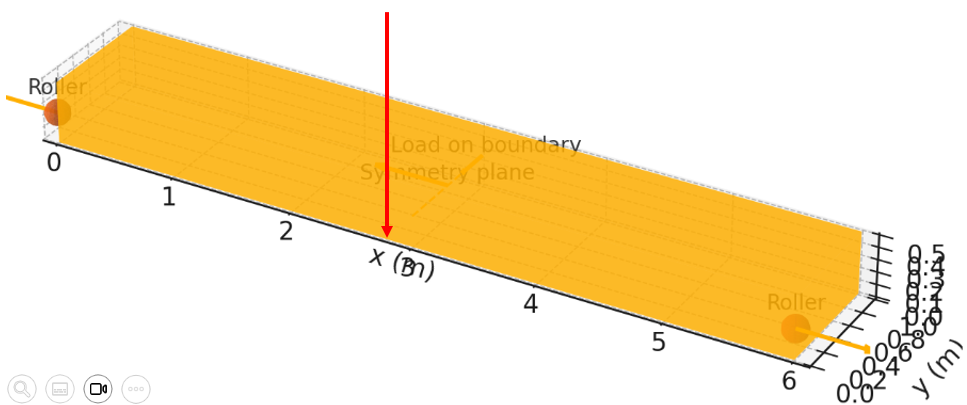
\includegraphics[width=0.9\textwidth]{2.png}
              \caption{Viga MBB}
              \label{fig:viga_mbb_ejemplo}
            \end{figure}

            \begin{figure}[H]
              \centering
              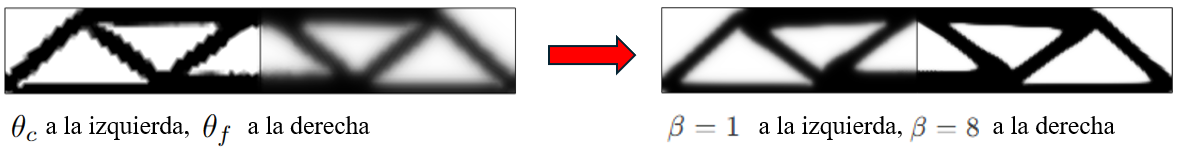
\includegraphics[width=0.9\textwidth]{1.png}
              \caption{Suavización y remodelamiento}
              \label{fig:suavizacion_remodelamiento}
            \end{figure}
          Entonces podemos notar que valores de $\beta$ altos hacen que la proyección sea más estricta y definida, mientras que valores bajos hacen que la función se asemeje a una función lineal y por eso seguiría viéndose difuminada. Por lo tanto, el valor de $\beta$ debe ser lo suficientemente alto para evitar la difuminación, pero no tan alto como para que la optimización no converja o que tenga mucho coste computacional.
          Además, para evitar que todo sea sólido, limitamos el volumen optimizado.
          \begin{equation}
            0 \leq \theta_{\mathrm{avg}} = \int\limits_{\Omega} \theta(\mathbf{x})\, d\Omega \leq V_{\mathrm{frac}}
          \end{equation}
            Para finalizar, garantizamos que la respuesta del modelo sea 0s y 1s. Aunque no puede faltar la inclusión de la rigidez en todo este cálculo, por tanto:
          \begin{equation}
            \theta_p = \theta_{\min} + (1 - \theta_{\min}) \theta(\mathbf{x})^p
          \end{equation}
          \begin{equation}
            E(\mathbf{x}) = E_0 \theta_p
          \end{equation}
          \section{Implementación en COMSOL}
          Para implementar el modelo en COMSOL, se debe crear un nuevo modelo y seleccionar el módulo de mecánica estructural. Luego, se debe definir la geometría de la viga MBB, que es un paralelepípedo de dimensiones $x = 6\,\mathrm{m}$ (largo), $y = 1\,\mathrm{m}$ (alto) y $z = 0.5\,\mathrm{m}$ (espesor). Después, se debe definir el material de la viga y las propiedades mecánicas necesarias, como el módulo de Young y la densidad. A continuación, se deben aplicar las condiciones de frontera y las cargas necesarias para simular el comportamiento de la viga bajo carga. Finalmente, se debe configurar el estudio de optimización topológica utilizando el método SIMP y los filtros necesarios.
\subsection{Definimos los estudios a realizar}
  \begin{figure}[H]
              \centering
              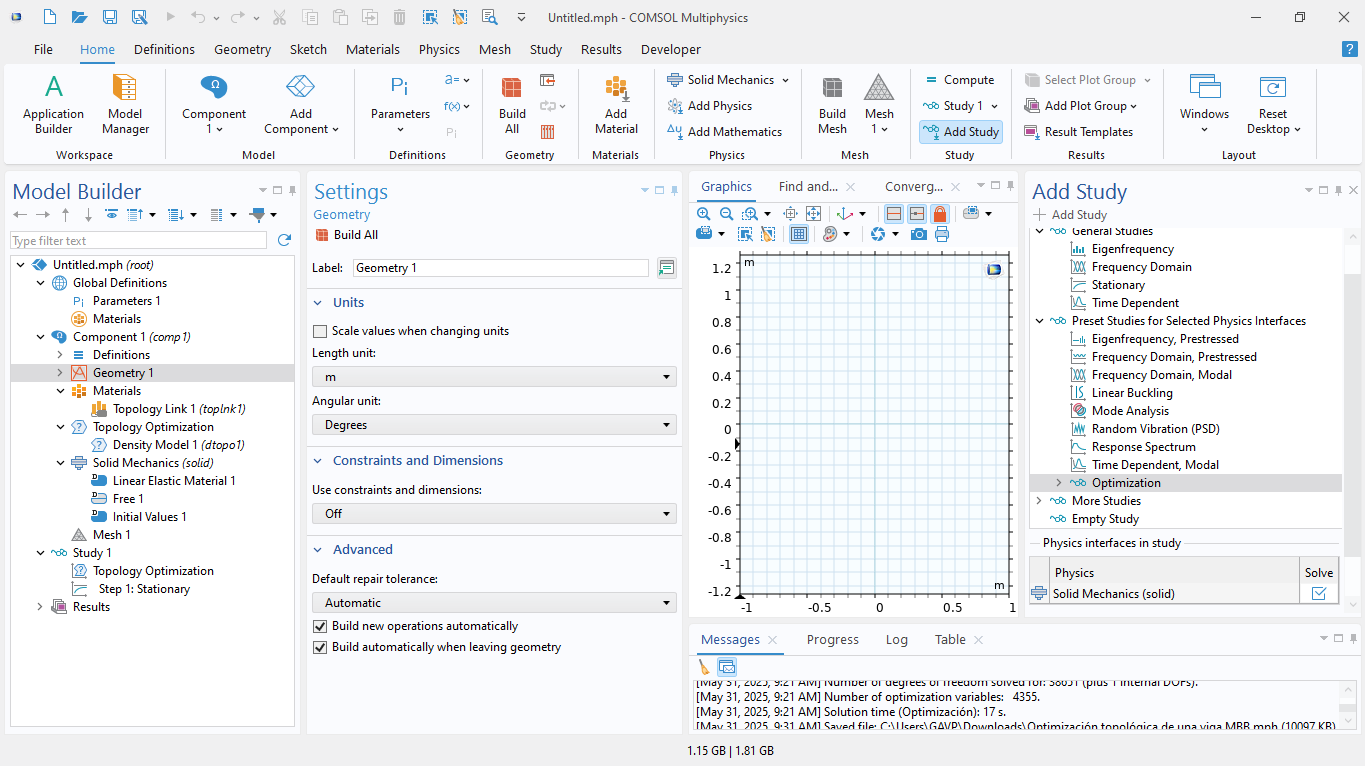
\includegraphics[width=0.9\textwidth]{Definimos los estudios a realizar.png}
              \caption{Model Solids and Topology Optimization Stationary}
              \label{fig:comsol_estudios}
            \end{figure}
\subsection{Definimos las variables mas importantes del estudio}
\begin{figure}[H]
              \centering
              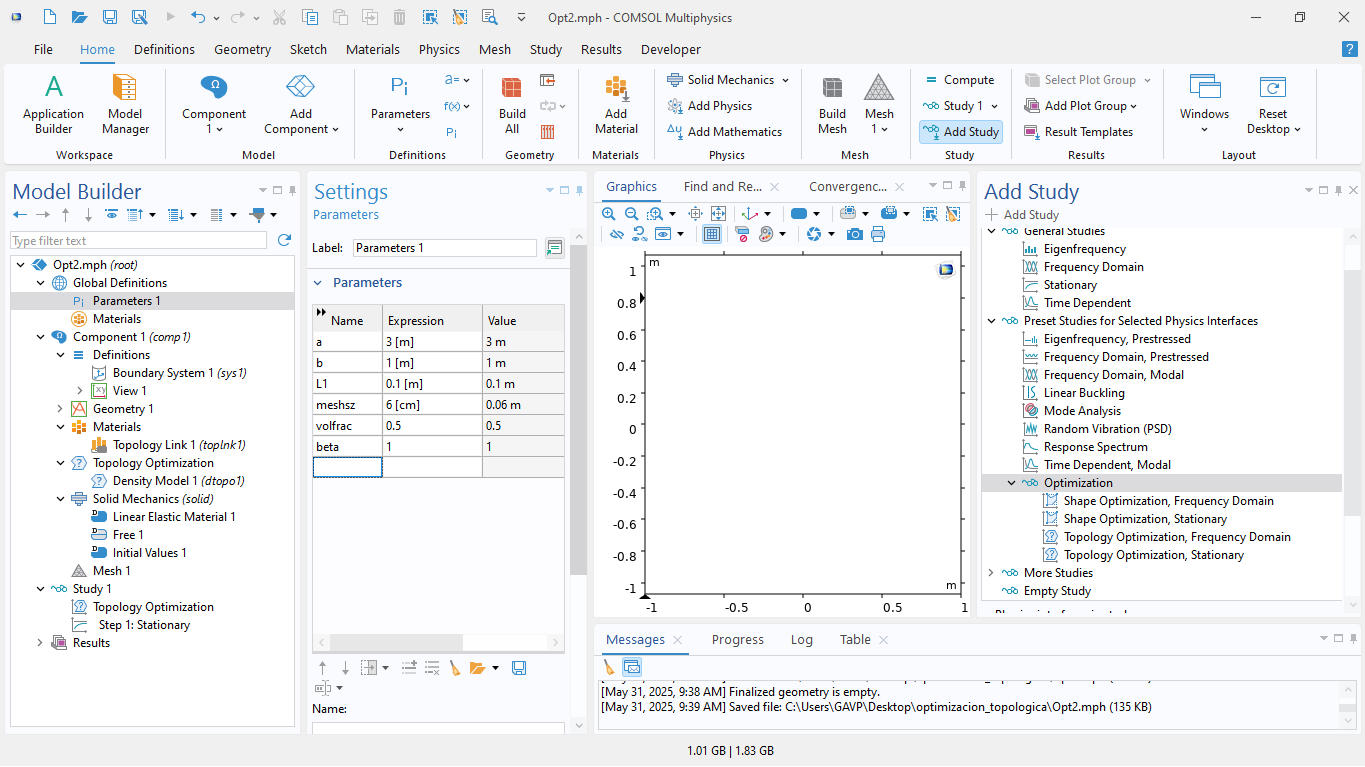
\includegraphics[width=0.9\textwidth]{variables.png}
              \caption{Definición de variables}
              \label{fig:comsol_variables}
            \end{figure}

            \subsection{Definimos la geometría a estudiar}
            \begin{figure}[H]
              \centering
              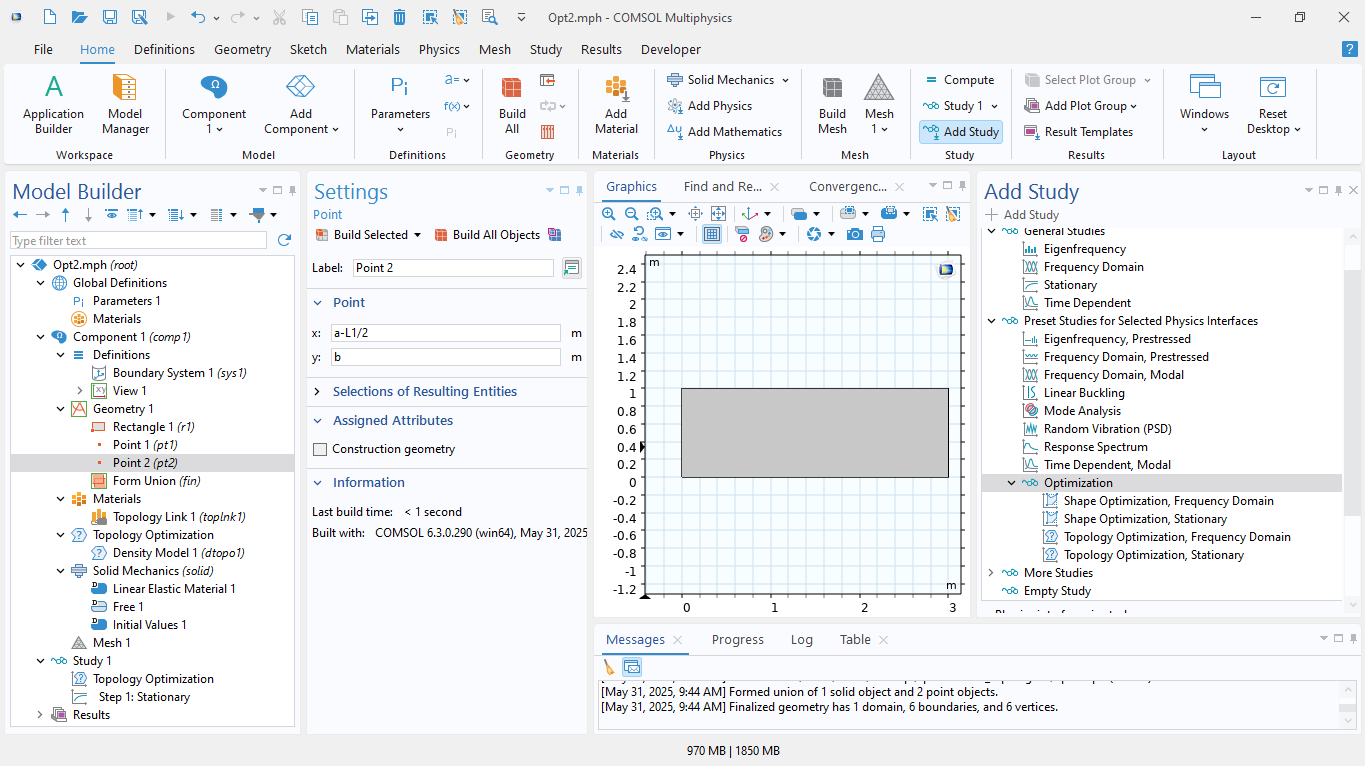
\includegraphics[width=0.9\textwidth]{Geaometria.png}
              \caption{Geometría rectangular}
              \label{fig:comsol_geometria}
            \end{figure}

            \subsection{Definimos los límites y simetrías}
             \begin{figure}[H]
              \centering
              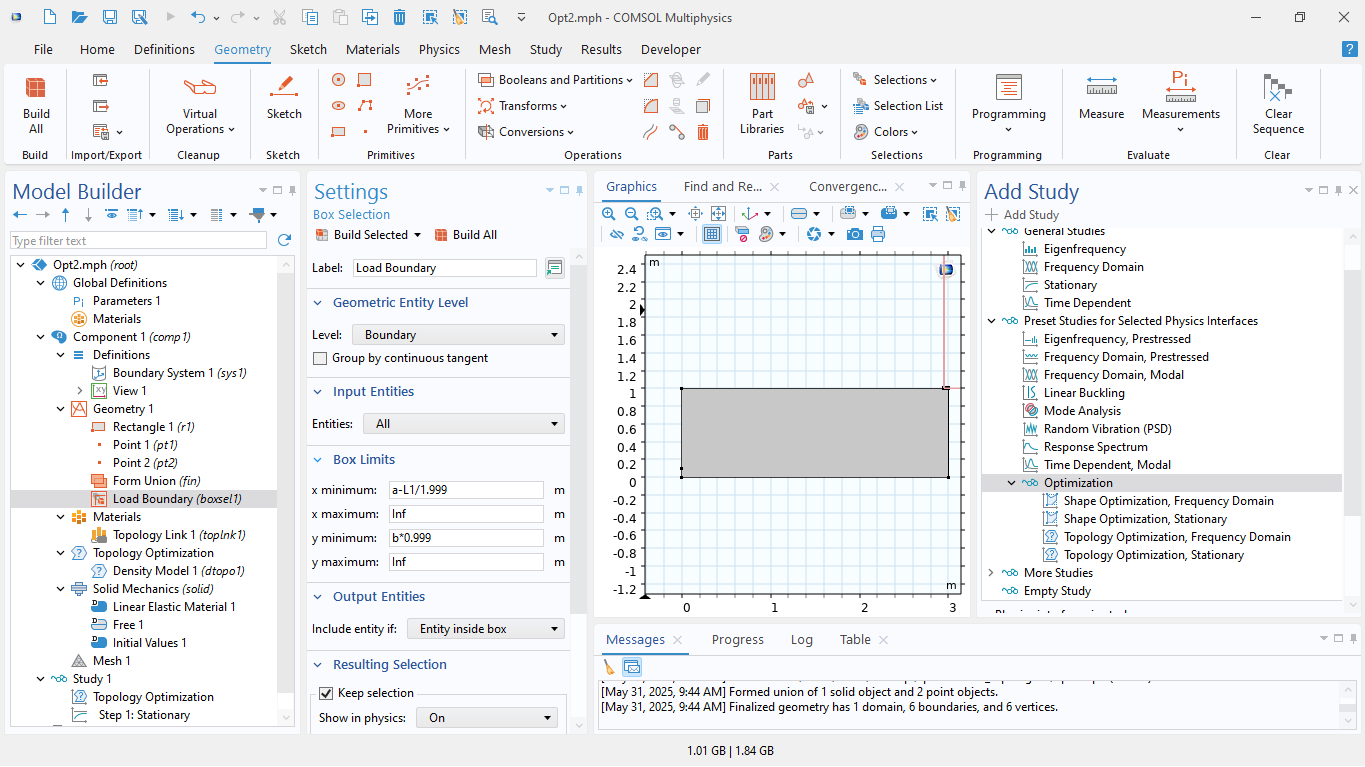
\includegraphics[width=0.9\textwidth]{Simetryy.png}
              \caption{Simetría en y}
              \label{fig:comsol_simetria_y}
            \end{figure}
              \begin{figure}[H]
              \centering
              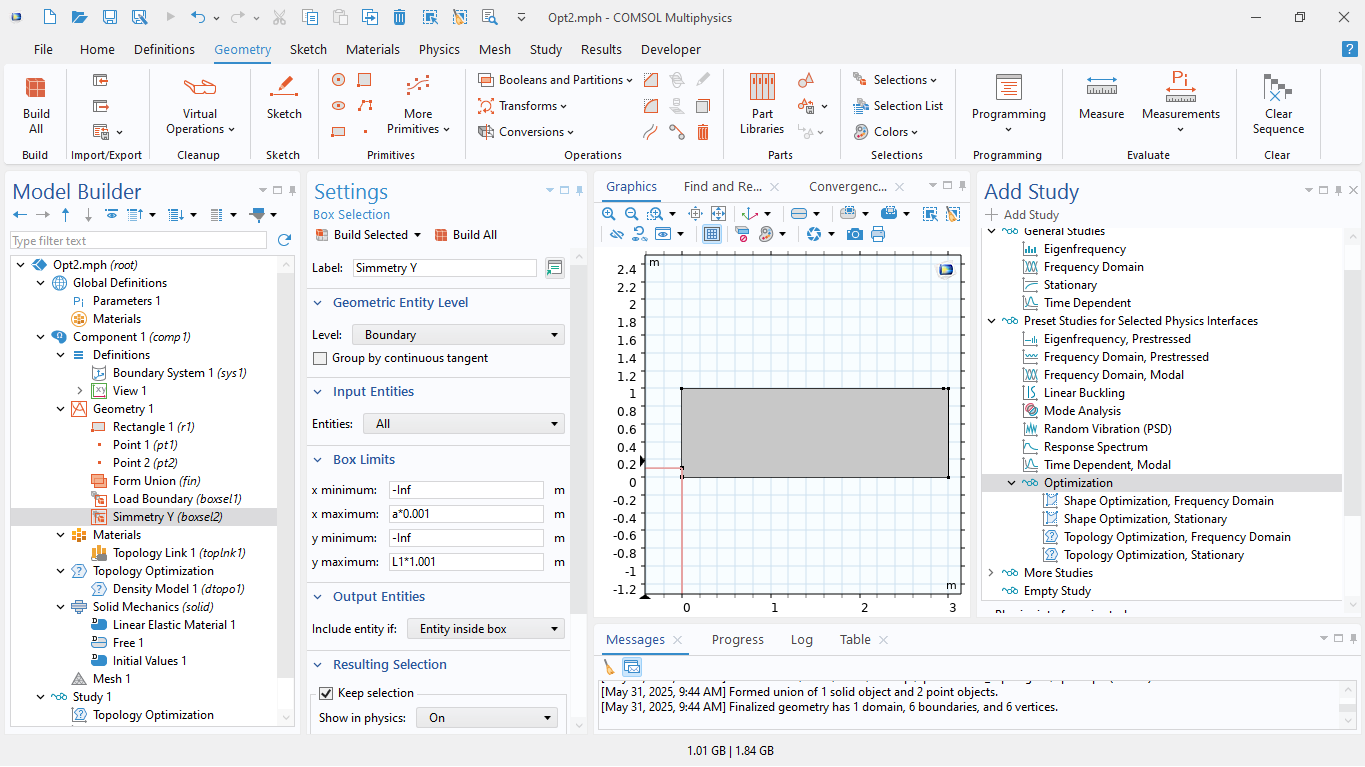
\includegraphics[width=0.9\textwidth]{Simetryy2.png}
              \caption{Simetría en x}
              \label{fig:comsol_simetria_x}
            \end{figure}
            \subsection{Agregamos el material}
             \begin{figure}[H]
              \centering
              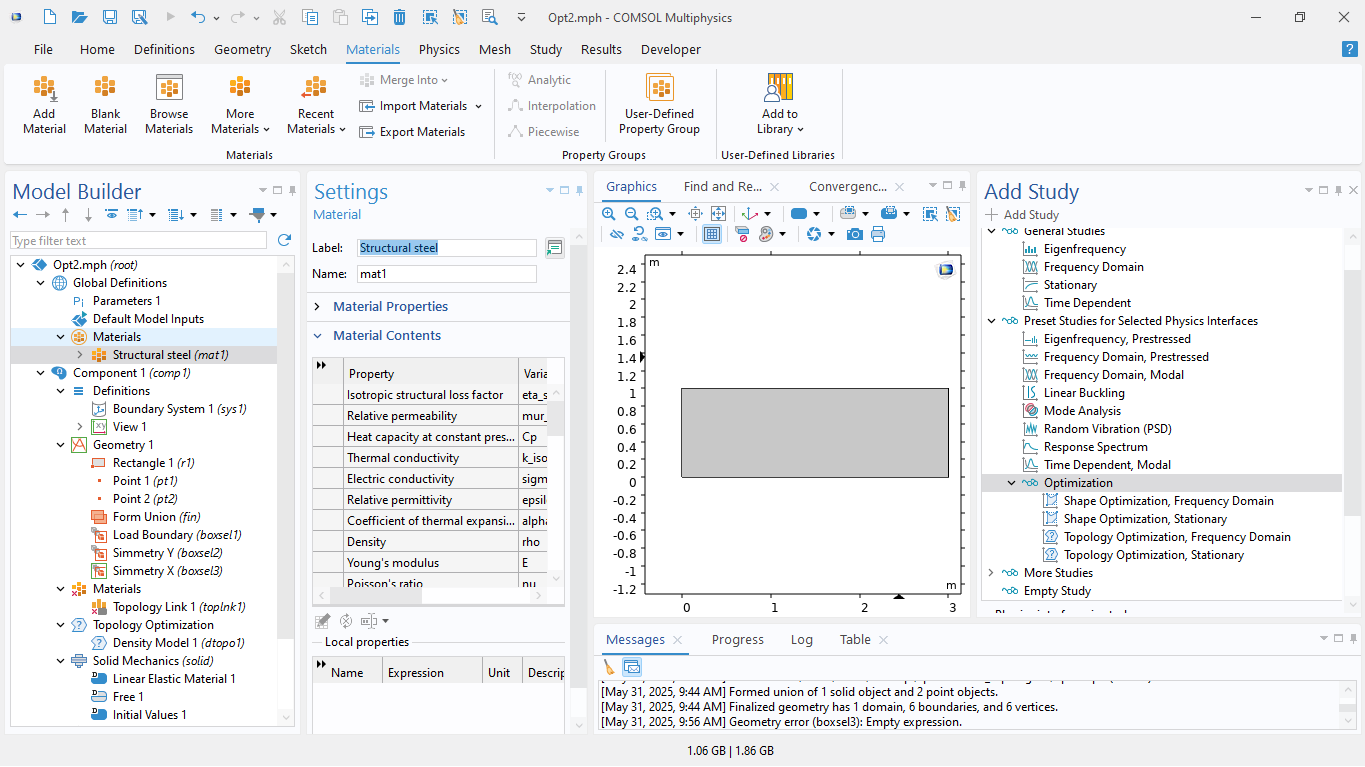
\includegraphics[width=0.9\textwidth]{mat.png}
              \caption{Structural Steel}
              \label{fig:comsol_material}
            \end{figure}
  \subsection{Agregamos los rollers y la fuerza}
  Definimos solo un roller ya que el otro llegará por simetría
             \begin{figure}[H]
              \centering
              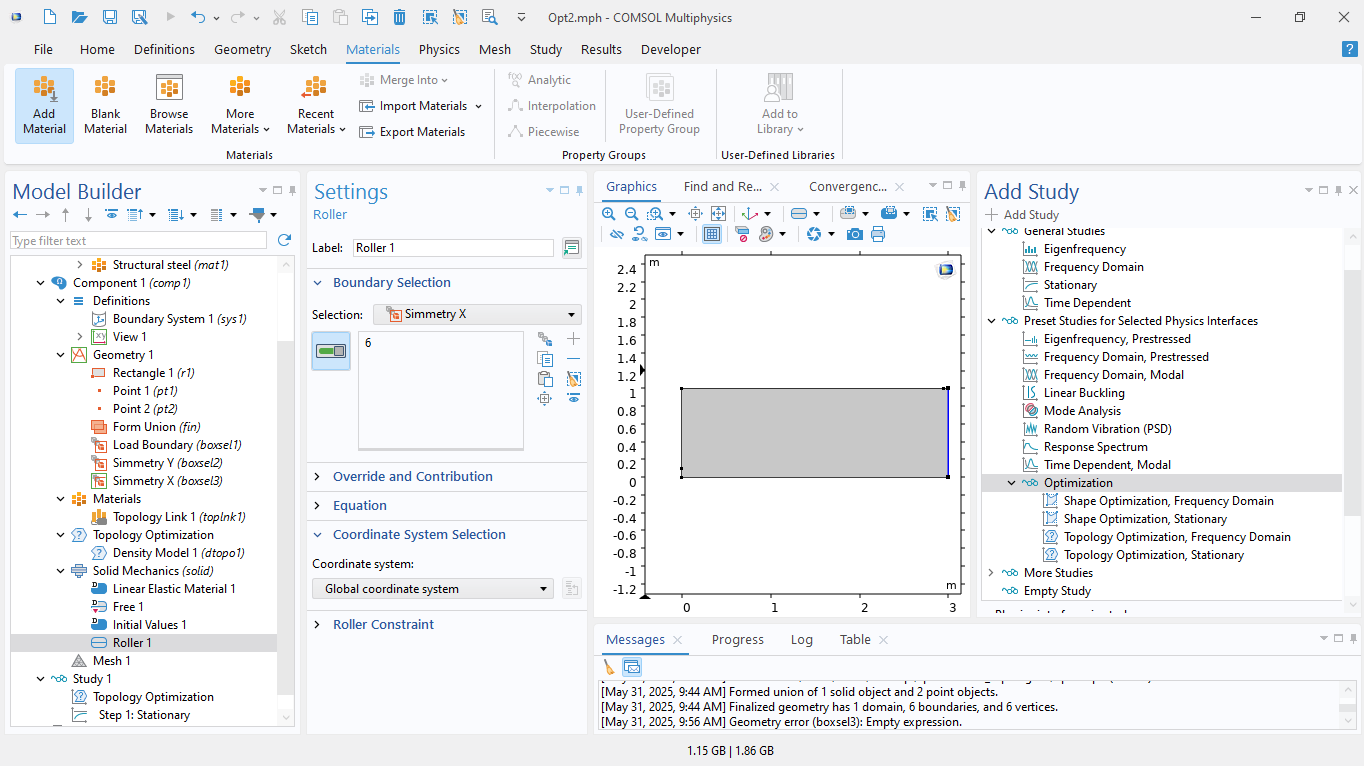
\includegraphics[width=0.9\textwidth]{roll1.png}
              \caption{Roller 1}
              \label{fig:comsol_roller1}
            \end{figure}

            \begin{figure}[H]
              \centering
              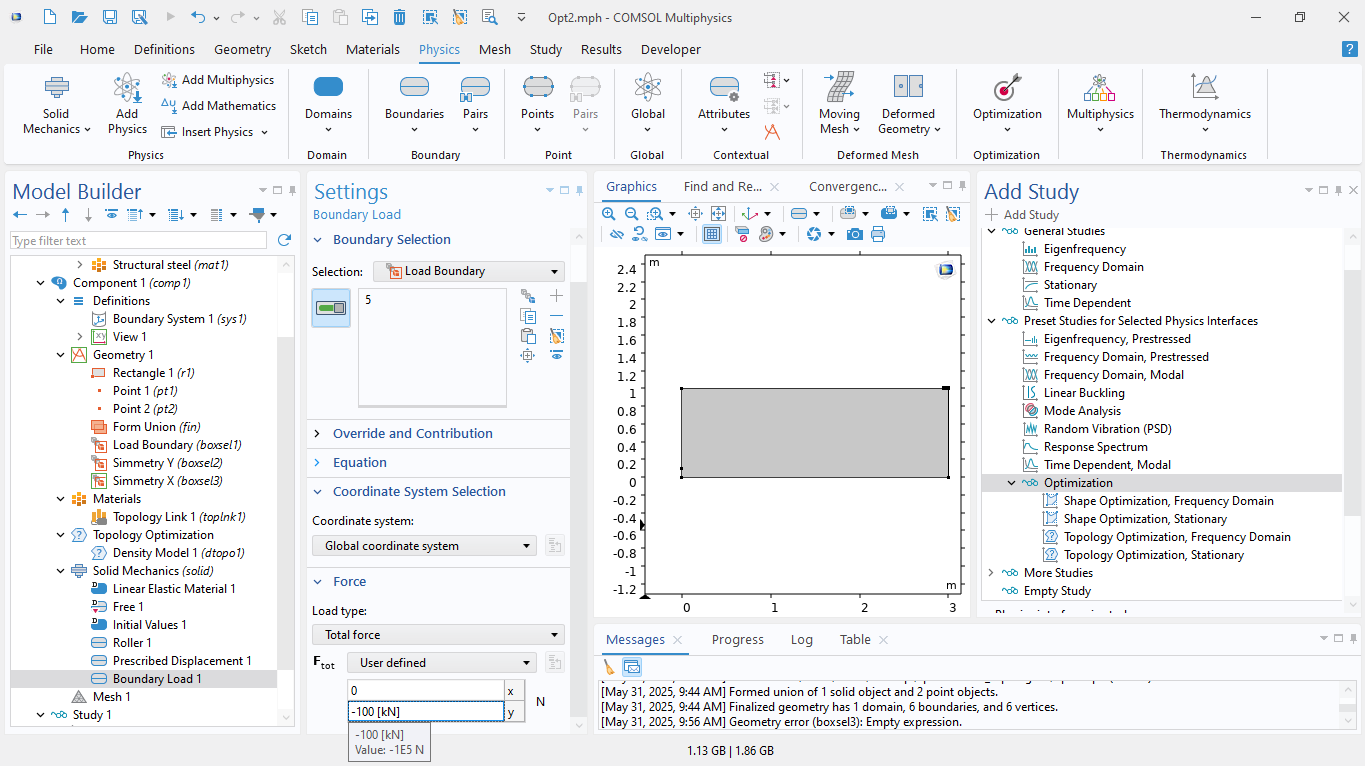
\includegraphics[width=0.9\textwidth]{force.png}
              \caption{Fuerza de -100 [kN]}
              \label{fig:comsol_fuerza}
            \end{figure}
\subsection{Definimos la malla}
             \begin{figure}[H]
              \centering
              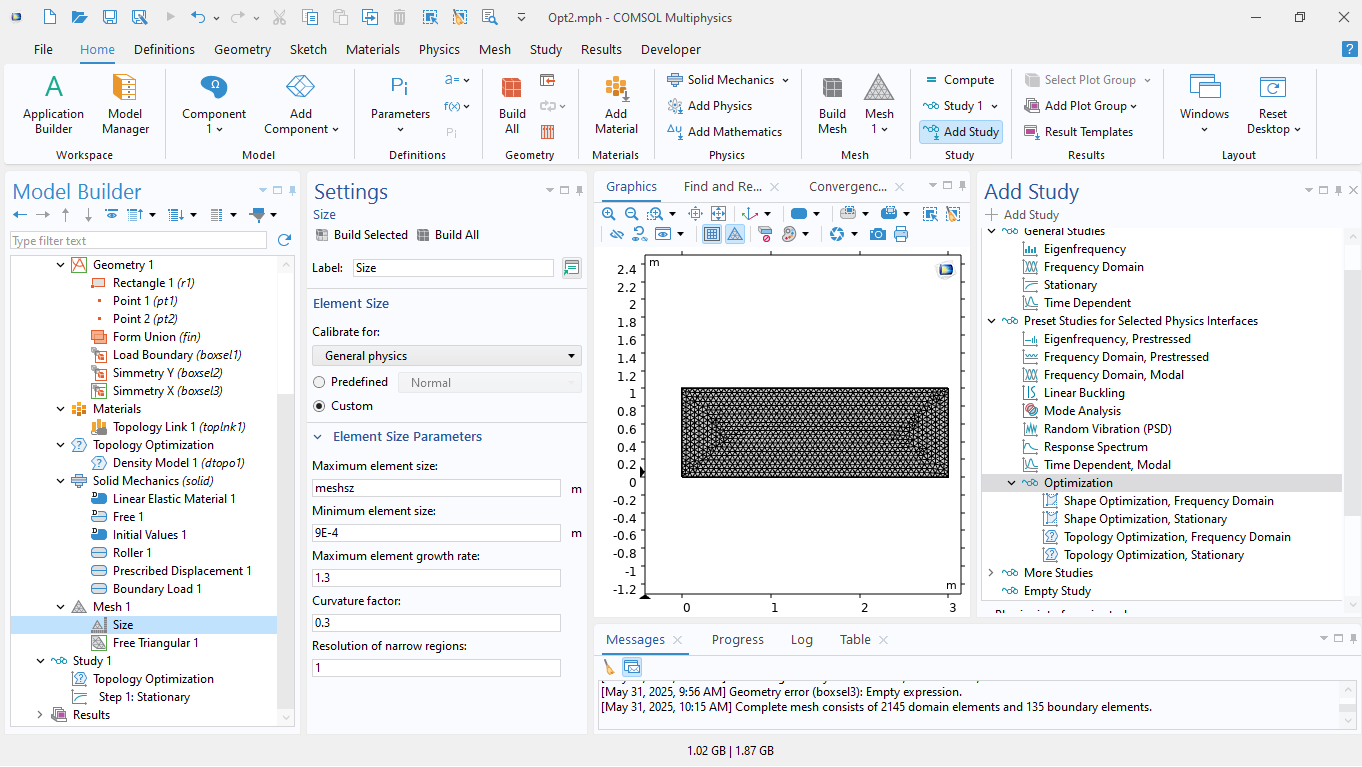
\includegraphics[width=0.9\textwidth]{malla.png}
              \caption{Malla}
              \label{fig:comsol_malla}
            \end{figure}

            \subsection{Parámetros para la optimización topológica}
             \begin{figure}[H]
              \centering
              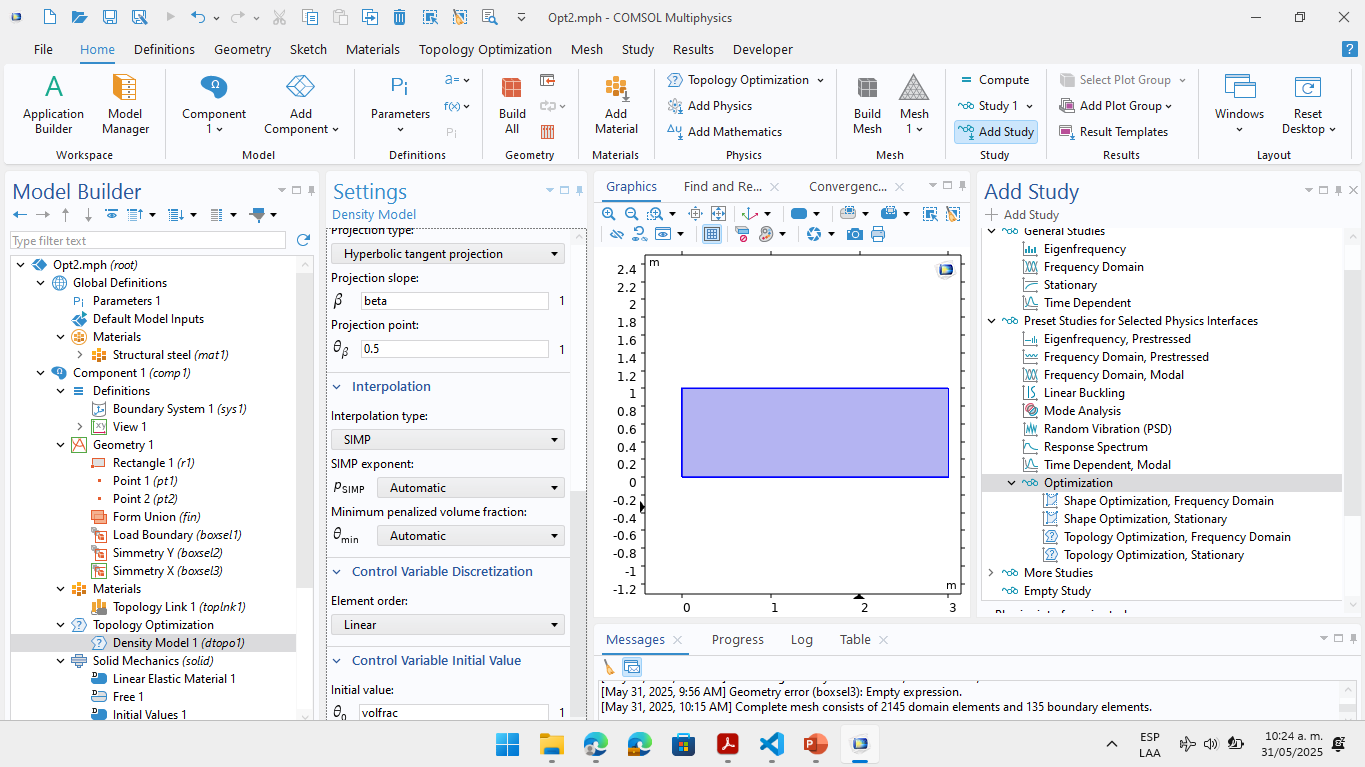
\includegraphics[width=0.9\textwidth]{opt.png}
              \caption{Optimización topológica}
              \label{fig:comsol_opt_topo}
            \end{figure}
              \begin{figure}[H]
              \centering
              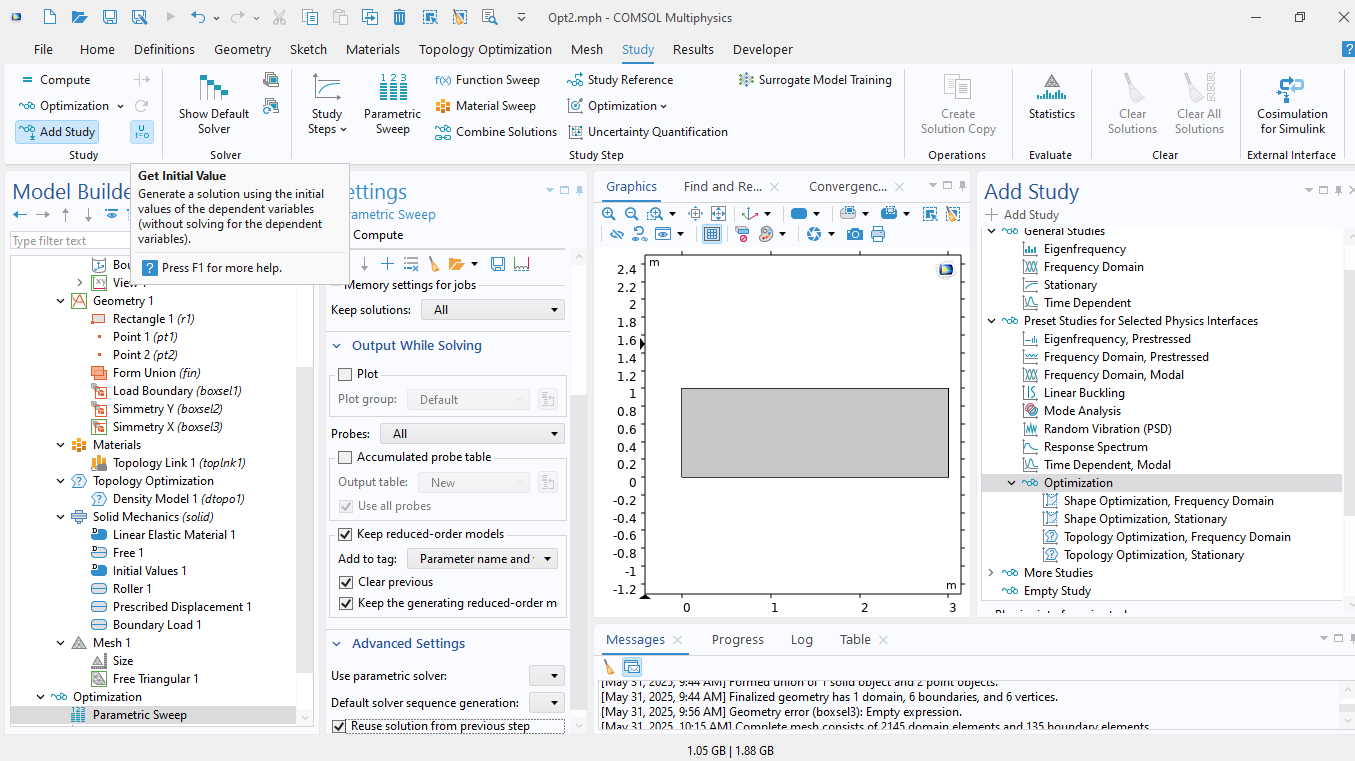
\includegraphics[width=0.9\textwidth]{Param.png}
              \caption{Parámetros Optimización topológica}
              \label{fig:comsol_opt_params}
            \end{figure}
            \begin{figure}[H]
              \centering
              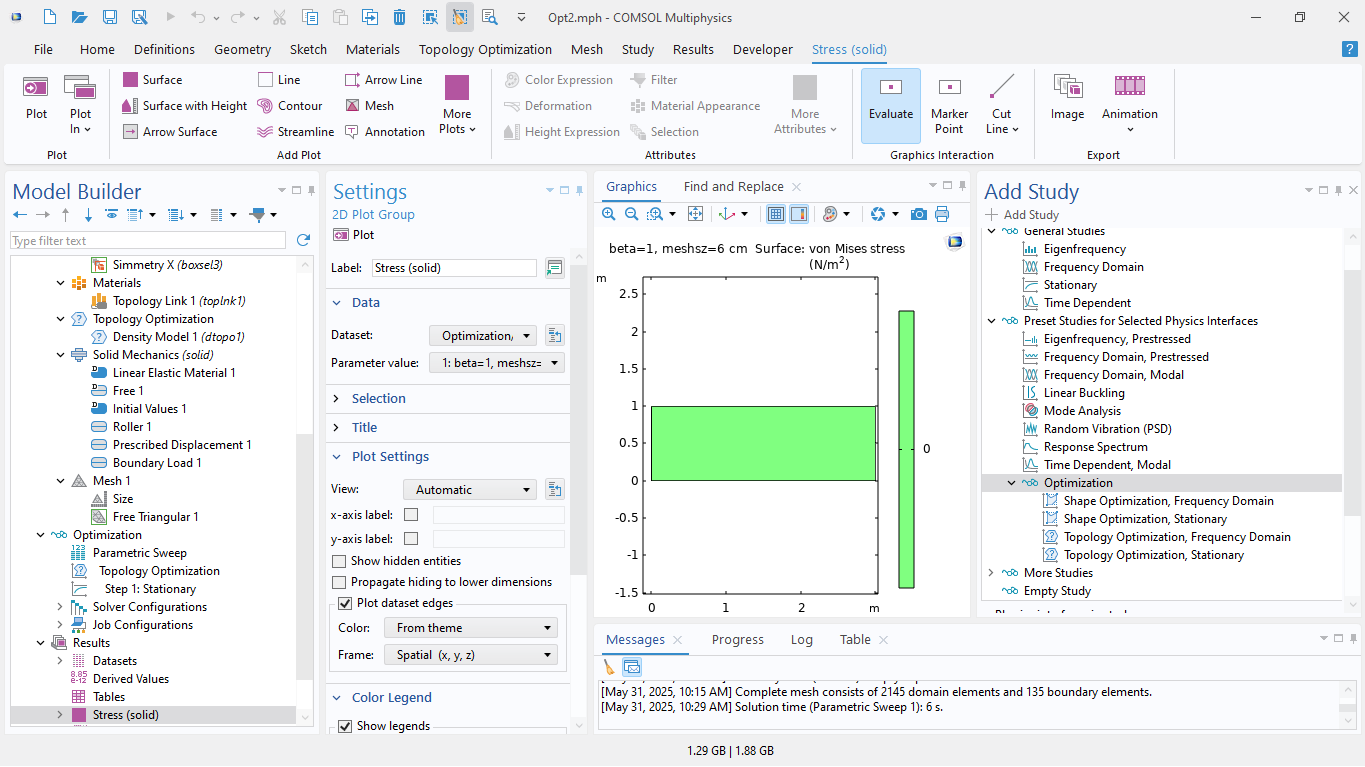
\includegraphics[width=0.9\textwidth]{initi.png}
              \caption{Get initial value}
              \label{fig:comsol_opt_initial}
            \end{figure}
            \subsection{Resultados y espejos}
             \begin{figure}[H]
              \centering
              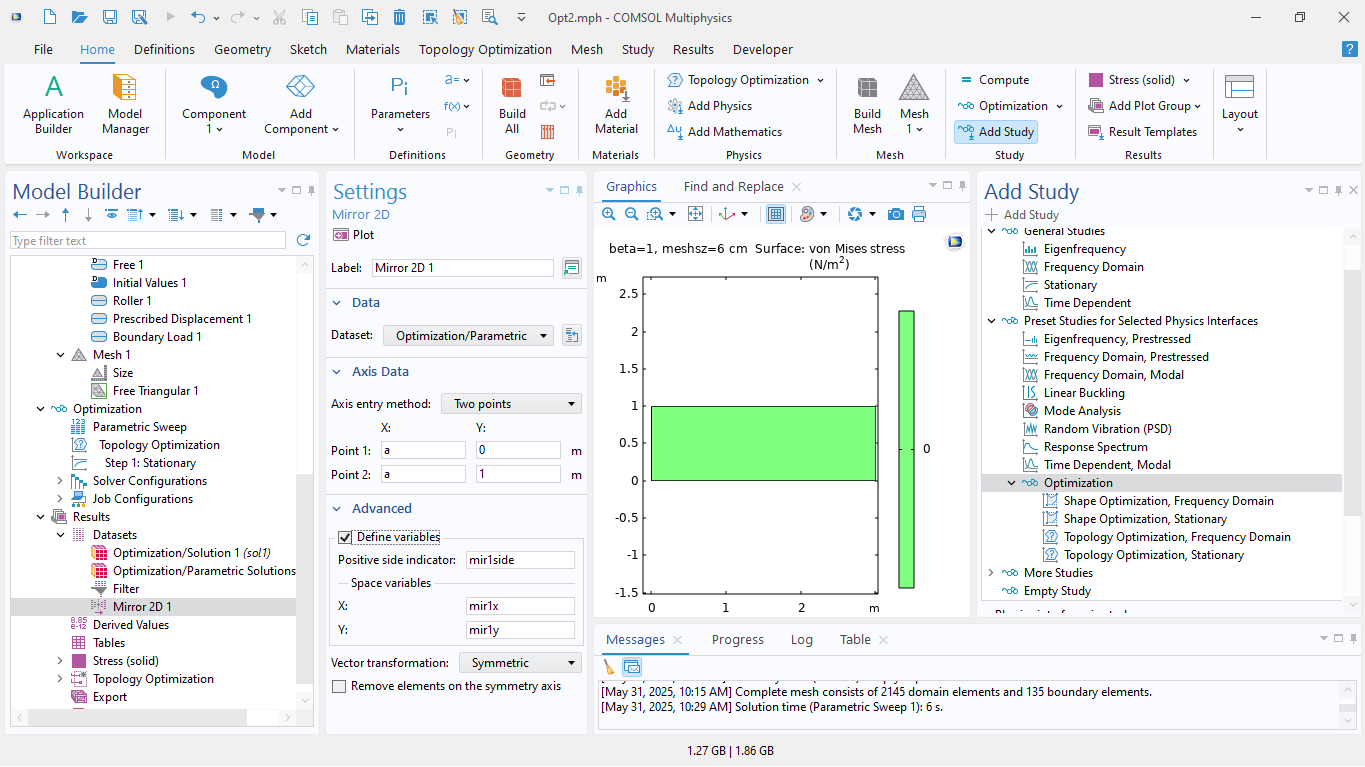
\includegraphics[width=0.9\textwidth]{mirror.png}
              \caption{Mirror 1}
              \label{fig:comsol_mirror1}
            \end{figure}

 \begin{figure}[H]
              \centering
              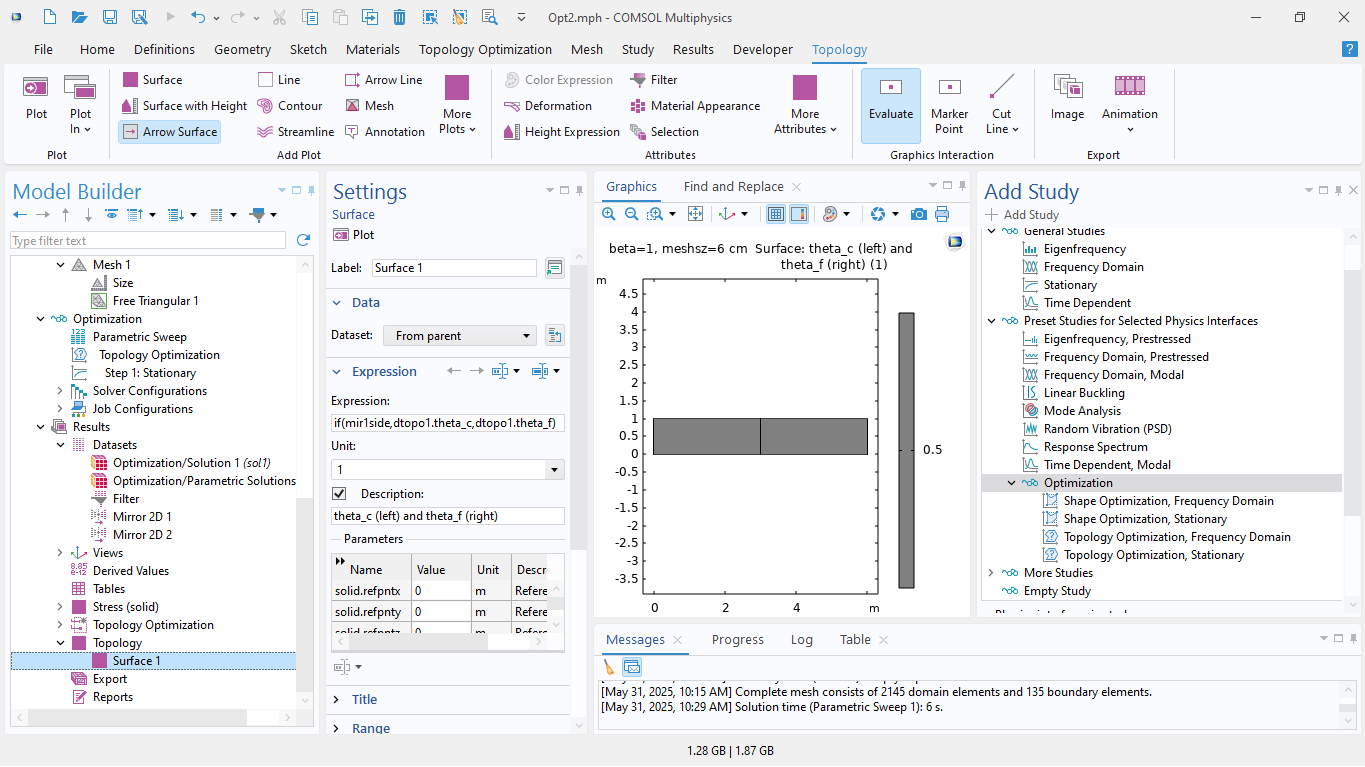
\includegraphics[width=0.9\textwidth]{sup.png}
              \caption{Superficie 1}
              \label{fig:comsol_superficie1}
            \end{figure}

             \begin{figure}[H]
              \centering
              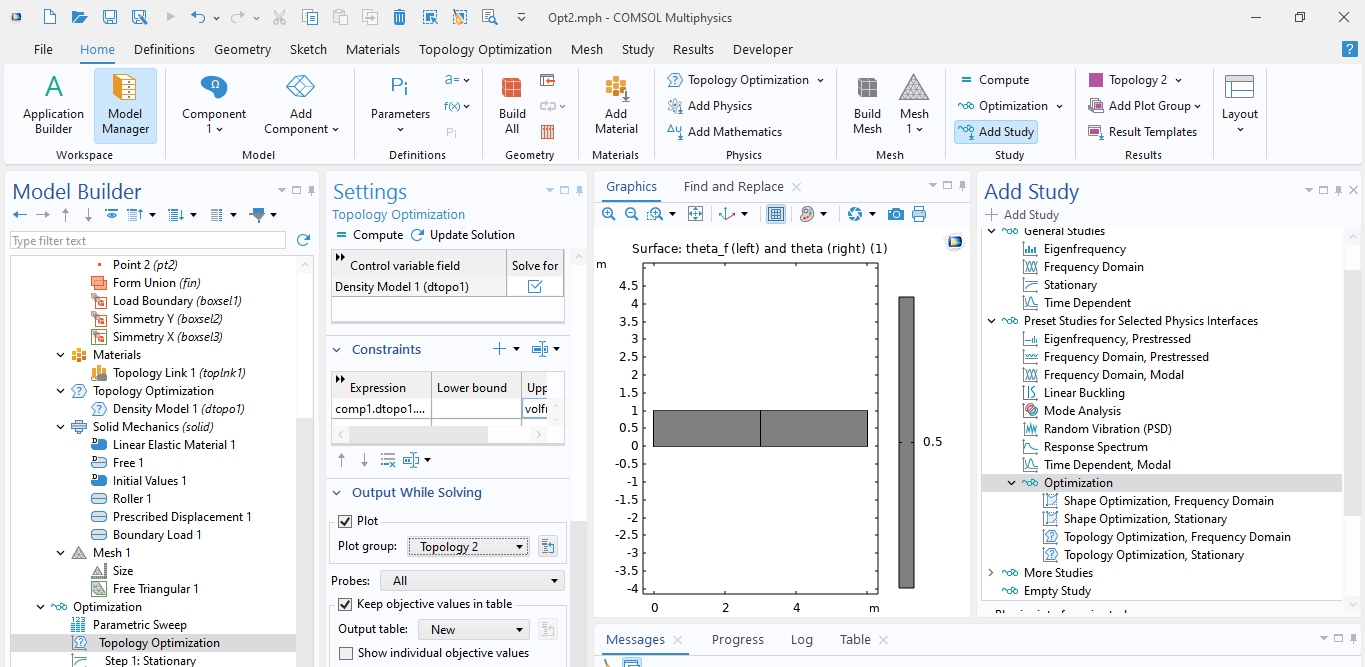
\includegraphics[width=0.9\textwidth]{las.png}
              \caption{Últimas configuraciones}
              \label{fig:comsol_ultimas_config}
            \end{figure}
\section{Resultados}
Los resultados obtenidos muestran una distribución óptima del material en la viga MBB, minimizando la masa mientras se cumplen las restricciones de carga y desplazamiento. La optimización topológica ha permitido identificar las áreas críticas donde se requiere mayor rigidez y, por lo tanto, se ha concentrado el material. El diseño final muestra una geometría eficiente que maximiza el rendimiento estructural.
 \begin{figure}[H]
              \centering
              \includegraphics[width=0.9\textwidth]{Distribución del esfuerzo.png}
              \caption{Distribución del esfuerzo}
              \label{fig:resultados_esfuerzo}
            \end{figure}
             \begin{figure}[H]
              \centering
              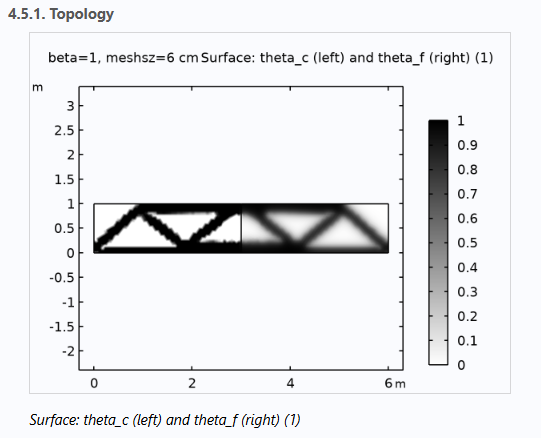
\includegraphics[width=0.9\textwidth]{Thetac.png}
              \caption{Thetac vs thetaf} 
              \label{fig:resultados_thetac_vs_thetaf}
            \end{figure}

            \begin{figure}[H]
              \centering
              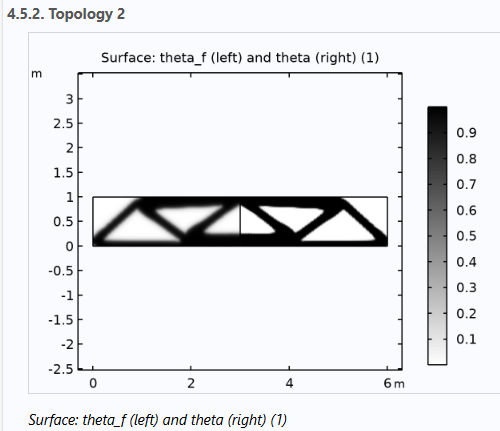
\includegraphics[width=0.9\textwidth]{theta.png}
              \caption{Thetaf vs theta} 
              \label{fig:resultados_thetaf_vs_theta}
            \end{figure}
          \section{Conclusiones}
La optimización topológica de la viga MBB utilizando el método SIMP ha demostrado ser una herramienta eficaz para mejorar el diseño estructural. Los resultados obtenidos indican que es posible reducir significativamente la masa del componente sin comprometer su integridad estructural. Además, la implementación en COMSOL Multiphysics ha facilitado el proceso de modelado y optimización, permitiendo una visualización clara de los resultados y una fácil interpretación de los datos. 
Además logramos comprobar todos los criterios de optimización mencionados anteriormente, como la suavización de la distribución del material, el control del volumen optimizado y la proyección de la variable de diseño. 

\bibliographystyle{apacite}
\nocite{*}
\bibliography{bib}
\end{document}